\section{Cross Validation} \label{ch:crossValidation}
Cross validation is used for evaluation the model. The cross validation is better for example residuals. The reason is that with the residuals they do not give an indication how well the model will predict with the new data that it did not show. One way to avoid this problem is to divide the data in several peace, in this case some data can be removed from training set to validate the model. This is the basic idea of cross validation. The cross validation best use is when we do not have test or validation data set or we have a small sample. There is several possibilities how can we perform cross validation some of them will be described below.

\section{Validation set approach}
\subsection{Theory}
The Validation set approach works by splitting the data to two parts one is called training set and the other is called testing set(validation or hold-out set). The model is tested with the training set, after the training is finished the model is tested with testing set which the model did not seen. From this testing we have test error, which is good for verifying the model. The plus of this method is low computation time, but the results of this method is heavily depended on which data point will end up in the sets.
\begin{figure}
	\centering
	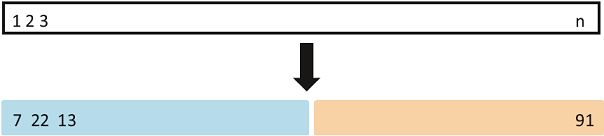
\includegraphics[width=0.4\linewidth]{crossValidation/validationSetApproach}
	\caption{Validation set approach. The entire dataset is split into a training and testing set}
	\label{fig:validationsetapproach}
\end{figure}

\subsection{Result}
In the lab 5.3.1 we used validation set approach to find the error. We are using auto data from the book. First of all we use the random seed to get the same results in the end. After words we spiting the the data set to two random subset of data.

\begin{lstlisting}[language=Python]
np.random.seed(1)
train = np.random.choice(data.shape[0], 196, replace=False)
select = np.in1d(range(data.shape[0]), train)

traindata = data[select]
\end{lstlisting}

Then we are fiting linear model on our training set and testing our model with the test data.

\begin{lstlisting}[language=Python]
import statsmodels.formula.api as smf
lm = smf.ols ('mpg~horsepower', traindata).fit() #Train the model on the traindata.

preds = lm.predict(data)
square_error = (data['mpg'] - preds)**2
print('--------Test Error for 1st order--------')
print(np.mean(square_error[~select]))
\end{lstlisting}
As we can see below the MSE is quit high.
\begin{lstlisting}

[1] Standard Errors assume that the covariance matrix of the errors is correctly specified.
--------Test Error for 1st order--------
23.36190289258723
\end{lstlisting}
We can reduce the MSE with polynomial or cubic regression.
\begin{lstlisting}[language=Python]
lm2 = smf.ols ('mpg~horsepower + I(horsepower ** 2.0)', traindata).fit()
preds2 = lm2.predict(data)
square_error2 = (data['mpg'] - preds2)**2
print('--------Test Error for 2nd order--------')
print(np.mean(square_error2[~select]))
lm3 = smf.ols ('mpg~horsepower + I(horsepower ** 2.0) + I(horsepower ** 3.0)', traindata).fit()
preds3 = lm3.predict(data)
square_error3 = (data['mpg'] - preds3)**2
print('--------Test Error for 3rd order--------')
print(np.mean(square_error3[~select]))
\end{lstlisting}
The out put:
\begin{lstlisting}[language=Python]
--------Test Error for 2nd order--------
20.25269085835005
--------Test Error for 3rd order--------
20.325609365773605
\end{lstlisting}
As we can see we are starting to reach the overfilling line with the cubic Polynomial. 
\section {K-fold cross validation}
\subsection{Theory}
In this typo of cross validation we split the data k-subsets and we repeat validation set approach for k times. In each time we take one subest as a test set and other combine are training set. After all copulations we compute average error. The advantage of this method is that all data points are one time in the testing set. The drift of the test is reduced when k is increasing. We can choose the k value, most oftenly k values are 5 or 10 . The disadvantages is that we have to retrain the model k times and the computation time increases. The mathematic formula is below. 
\begin{align}\label{fo:k-fold}
CV_{(K)} = \sum_{k=1}^{K}  \frac {n_{k}}{n}MSE_{(k)}
\end{align}

\subsection{Result}
In the lab 5.3.3 we used K-fold cross validation find the MSE. We are using auto data from the book. In this particular case we are using k = 10. 
\begin{lstlisting}[language=Python]
from sklearn.model_selection import KFold

X = Data["horsepower"].values.reshape(-1,1) 
y = Data["mpg"].values.reshape(-1,1)
kf= KFold()
kf.n_splits = 10
\end{lstlisting}
Now we need to make a loop for all the folds to calculate MSE.   

\begin{lstlisting}[language=Python]
ytests = []
ypreds = []

for train_index, test_index in kf.split(Data):
	X_train, X_test = X[train_index], X[test_index]
	y_train, y_test = y[train_index], y[test_index]

	model = linear_model.LinearRegression()
	model.fit(X = X_train, y = y_train)
	y_pred = model.predict(X_test)  
	ypreds += list(y_pred)
	ytests += list(y_test)
	ms_error = metrics.mean_squared_error(ytests, ypreds)
	print("%.2f" %ms_error, end=" ")
\end{lstlisting}
Out put of the code is:
\begin{lstlisting}[language=Python]
28.35 22.79 24.14 23.95 22.29 21.56 20.92 21.16 26.11 27.42 
\end{lstlisting}
Having all MSE we can choose the best model from the results. or 

\section {Leave one out cross validation}

\subsection{Theory}
This type of cross validation is used when there is limited amount of data. It works the same way as k-fold cross validation, but instead subset we are using signal data entry, that means K is N in this case.The mathematic formula is below. 

\begin{align}\label{fo:LOOCV}
CV_{(n)} = \frac {1}{n} \sum_{k=1}^{K}  (\frac {y_i-\hat{y_i}}{1- h_i})^2
\end{align}
\subsection{Result}
In lab 3.4.2 we had the same auto data. We used the LOOCV method to find MSE. We made an algorithm for this method, because we coul not find a library for this method.

\begin{lstlisting}[language=Python]
X = df["horsepower"].values.reshape(-1,1)
y = df["mpg"].values.reshape(-1,1) 

loo = LeaveOneOut()
print('Splits: ', loo.get_n_splits(X))

ytests = []
ypreds = []

for train_index, test_index in loo.split(X):
	X_train, X_test = X[train_index], X[test_index]
	y_train, y_test = y[train_index], y[test_index]

	model = linear_model.LinearRegression()
	model.fit(X = X_train, y = y_train)
	y_pred = model.predict(X_test)

	ytests += list(y_test)
	ypreds += list(y_pred)
	
rr = metrics.r2_score(ytests, ypreds)
ms_error = metrics.mean_squared_error(ytests, ypreds)

print("LOOCV results:")
print("R^2: {:.5f}%, MSE: {:.5f}".format(rr*100, ms_error))
\end{lstlisting}

The output:
\begin{lstlisting}[language=Python]
Splits:  392
LOOCV results:
R^2: 60.12110%, MSE: 24.23151
\end{lstlisting}

As we can see our algorithm has worked.Also we have seen a mass increased computing time in the machine. It was expected, because of retraining and revalidating the model 392 time.




